\documentclass[12pt, letterpaper]{article}
\usepackage[utf8]{inputenc}
\usepackage{fancyhdr}
\usepackage{graphicx}

\usepackage{enumitem}
\usepackage{float}

\graphicspath{ {./images/} }

% Title Page
\title{Software Development Project - 1DV600}
\author{Claes Weyde}

\pagestyle{fancy}
\fancyhf{}
\fancyhead[L,R]{The Marvelous Hanging Man}
\fancyhead[R,L]{Claes Weyde}
\fancyfoot[C,C]{\leftmark}
\fancyfoot[L,R]{\thepage}
\fancyfoot[R,L]{Version 3.0}



\begin{document}
\maketitle
\newpage
\tableofcontents{}
\newpage

\section{Revision history}
\begin{center}
	\begin{tabular}{|c|c|c|c|} 
		\hline
		Date & Version & Description & Author \\ [0.5ex] 
		\hline\hline
		05.02.2019 & Version 1.0 & Skeleton document provided & Claes Weyde \\
		\hline
		06.02.2019 & Version 1.1 & Vision, first draft of project plan section & 
		Claes Weyde \\
		\hline
		07.02.2019 & Version 1.2 & Project plan finished & Claes Weyde \\ [1ex] 
		\hline
		07.02.2019 & Version 1.3 & General information finished & Claes Weyde \\
		\hline
		07.02.2019 & Version 1.4 & Iteration and Risk analysis & Claes Weyde \\ 
		\hline
		14.02.2019 & Version 2.0 & Detail planning Iteration 2 & Claes Weyde \\
		\hline
		14.02.2019 & Version 2.1 & Updated time log after UML work & Claes Weyde \\
		\hline
		21.02.2019 & Version 2.2 & Updated time log after implementation work & Claes Weyde \\
		\hline
		21.02.2019 & Version 2.3 & Updated time log for class diagram & Claes Weyde \\
		\hline
		21.02.2019 & Version 2.4 & Reflection writing & Claes Weyde \\
		\hline
		02.03.2019 & Version 3.0 & Updated iteration 3 & Claes Weyde \\
		\hline
		17.03.2019 & Version 3.1 & Planned iteration 4 in detail & Claes Weyde \\
		\hline
		20.03.2019 & Version 3.2 & Wrote some test case information & Claes Weyde \\
		\hline
		21.03.2019 & Version 3.2 & Finalized the document & Claes Weyde \\
		[1ex]
		\hline
		
	\end{tabular}
\end{center}
\newpage
\section{General Information}
\begin{tabular}{ |c|c|  }
	\hline
	\multicolumn{2}{|c|}{\textbf{Project Summary}} \\
	\hline
	\textbf{Project Name} & \textbf{Project ID} \\
	\hline
	The Marvelous Hanging Man & HM-001 \\
	\hline
	\textbf{Project Manager} & \textbf{Main client} \\
	\hline
	Claes Weyde & Language learners   \\
	\hline
	\multicolumn{2}{|c|}{\textbf{Key Stakeholders}}\\
	\hline
	\multicolumn{2}{|l|}{Developing team, main client/end user}\\
	\hline
	\multicolumn{2}{|c|}{\textbf{Executive summary}}\\
	\hline
	\multicolumn{2}{|l|}{Developing a text and ASCII-art based game of hangman for}\\
	\multicolumn{2}{|l|}{the language learner, as well as for the gamer looking for}\\
	\multicolumn{2}{|l|}{a cognitive challenge.}\\
	\multicolumn{2}{|l|}{The project will be split up into a planning phase, a modeling}\\
	\multicolumn{2}{|l|}{ and implementation phase, a testing phase and an}\\
	\multicolumn{2}{|l|}{ evolutionary phase.}\\
	\multicolumn{2}{|l|}{The project is planned to take about 7 weeks and the  }\\
	\multicolumn{2}{|l|}{complete application will be delivered on the 22 of March 2019.}\\

	\hline
	
\end{tabular}
\newpage
\section{Vision}
Hangman re-imagined! Our vision for this project is to create a version of Hangman which will keep the user at the edge of her or his seat. To not only provide entertainment and leisure, but also thought-provoking imagery and themes. 
\newline
\newline
 The Hangman game we envision will be a text-based console application where the user will play hangman. The end user we primarily envision is a person learning a new language or trying to increase their grasp of a language which they already know. By making the process fun we believe that learning is facilitated and that the user will have a easier time recalling the material. However, the game is not only aimed at language learners but also to the casual player looking for a bit of fun.
 \newline
 \newline
 To aid learning and encourage competitiveness (which may be a means for aiding learning) a high-score system should be implemented, giving the user the possibility of competing against him or herself and other users. Furthermore, we also envision the usage of incentives for the user who performs well. The high-score is certainly one, but another may be the possibility of adding new words to the game. Thereby the well-performing user have the ability of evolving the game further. To cater to different users, as well as to allow the avid user to constantly evolve, we also envision the possibility for the player to choose a difficulty.
 \newline
 \newline
  In short, we aim to deliver a game where fun and learning combine in an intuitive end product!
  \subsection{Reflection}
  It is hard to provide a vision at such an early phase and for such a bare-bones project without adding all the bells and whistles I can imagine. It would certainly be possible (and fun) to add more and more functionality in the vision, but somewhere the rubber must meet the road, and my goal is to have to remove as few features as possible when that happens. Therefore I tried to keep the vision as realistic as possible given what time I have at my disposal. Since this is one of the first sections I write I feel that my grasp on the project is tenuous at best, which is why my main goal is to provide a vision with a high probability of success. Perhaps at the cost of any chances for a bestselling application.  


\newpage 
\section{Project Plan}
\subsection{Introduction}
The aim of this project is to develop a game of hangman which fulfills as many of the properties specified in the vision above as possible, within the time available for the course.
\subsection{Justification}
The justification for this application is, at the most superficial level, that it is required in order to pass the course 1DV600. However, a deeper, and most probable more important justification is that the development of this application as well as the documentation will help me become a better developer with a deeper understanding of the project of development, i.e. not just the coding but planning, implementation, testing and (perhaps to a lesser extent) maintenance. Furthermore, the game itself may be justified in this day and age by the (at least anecdotally) reduced spelling capabilities of the population, which may stem from the ubiquitous auto-correct functionality used whenever we write. 
\subsection{Stakeholders}
The stakeholders for this project are listed below.
\begin{itemize}
	\item Management - The management want a product according to their specifications and budget. The management will evaluate the iterations of the product as well as the end-product with a view to costs and possible revenue.
	\item Project Manager - The project manager is ultimately responsible for the success of the project. Thus, the project manager will focus on the processes, timetables and workings of the group in order to ensure that the project is successfully completed. 
	\item Developer - The person or team performing the actual work of coding the software. The main focus of the developer is to arrive at an executable application of the game, i.e. a playable hangman application.
	\item Test lead - the person responsible for the validation of the software. The main focus of the test lead will be to ensure that the software does not contain any bugs and works according to the specifications.
	\item End user - the person(s) that will use the application. The main perspective of the end user is that the experience of using the application is enjoyable and perhaps efficient (depending on the type of application). Since this project is a game the end user most probably is looking for a fun experience, something which he/she wants to do during their downtime. The end user envisioned here is primarily the language learner looking for a fun software to increase their spelling proficiency. 
\end{itemize}
The author of this document will take on the roles of both project manager, developer and test lead.
\subsection{Resources}
The resources used to develop this application and documentation are as follows.
\begin{itemize}
	\item Hardware: a custom desktop computer and a Lenovo laptop computer are used for this project.
	\item Software
	\begin{itemize}
		\item Documentation: TeXStudio is used in conjunction with MikTex in order to produce the documentation.
		\item Application: The application is written in Visual Studio Code using Node.
	\end{itemize}
	\item Time: The time available for the project ranges between 6 and 15 hours/week.
\end{itemize}
\subsection{Hard- and Software Requirements}
The hardware requirements for this application will be very low. The application will be guaranteed to run on a computer having:
\begin{itemize}
	\item Hardware
		\begin{itemize}
		\item At least 1 GB RAM
		\item CPU having a frequency of 1.1 GHz and higher.   
	\end{itemize}
	\item Software
	\begin{itemize}
		\item Operating system: Win 7 or greater, OS X 10.7 or greater.
	\end{itemize}
\end{itemize} 
\subsection{Overall Project Schedule}
\begin{center}
	\begin{tabular}{|c|c|c|} 
		\hline
		Iteration & Deliverable & Date \\ [0.5ex] 
		\hline\hline
		Iteration 1 & Documentation draft 1  & 08.02.2019 \\ 
		\hline
		Iteration 1 & Skeleton Code & 02.08.2019 \\
		\hline
		Iteration 2 & Documentation draft 2 & 22.02.2019  \\
		\hline
		Iteration 2 & UML documentation & 22.02.2019  \\
		\hline
		Iteration 2 & Working code implemented & 22.02.2019  \\
		\hline
		Iteration 3 & Documentation draft 3 & 08.03.2019  \\
		\hline
		Iteration 3 & TBD (testing) & 08.03.2019  \\
		\hline
		Iteration 4 & Complete documentation & 22.03.2019  \\
		\hline
		Iteration 4 & Complete project & 22.03.2019  \\ [1ex] 
		\hline
	\end{tabular}
\end{center}
\subsection{Scope, Constraints, Assumptions}
\subsubsection{Scope}
The scope of the project will now be delimited by the functional requirements set forth below.
\begin{itemize}
	\item \textbf{UI} The user interface will be text-based, thus no GUI will be developed.
	\item \textbf{Menu} The application will have a starting menu consisting of:
	\begin{itemize}
		\item \textbf{Login} Where the user can log in to use a saved account.
		\item \textbf{Difficulty} Where the user can set the difficulty level of the game.
		\item \textbf{High-score} Where the user can see the current high scores.
		\item \textbf{Manage words} Where a "super user" can remove and add words to the game. The "super user" will be a logged in user having special authorization. Thus, this choice cannot be made by regular users. Alternatively a special password will be required in order to access this menu item.
		\item \textbf{Play} - Where the user can start a new game.
	\end{itemize}
	\item \textbf{Difficulty} The game will have at least three difficulty levels: easy, moderate and hard. The difficulty level chosen will determined the words drawn and the number of incorrect letters the user may write. As a starting point the number of incorrect letters will be 3 for hard, 5 for moderate and 7 for easy. The words drawn may be determined based on the number of letters contained within the word. Alternatively the difficulty of the words may be a property or characteristic of the word which is set when the word is first saved. This property may also be adjustable in the manage words category of the menu.
	\item \textbf{High-scores} The 10 highest score for each difficulty will saved. The score will be based on the amount of words successfully completed before the user quit or lost the game. The player loses the game when the man is hanged.
	\item \textbf{Timer} A timer will be implemented which keeps track of the time used for each word. The mean may be determined and shown if the game makes it to the high-score. The running time will be shown as the player plays the game.
	\item \textbf{Adding words} If the user achieves a high-score he/she will have the possibility of adding a word to the words of the game.
	\item \textbf{Managing words} The super user (or the user having the right password depending on the implementation) will be able to manage the words by choosing this option in the menu. The user should have the ability to remove words, add words as well as changing the words and their difficulty assessment.
	\item \textbf{Graphics} The hanged man will be shown using ASCII-art.
\end{itemize}
\subsubsection{Constraints}
The constraints are itemized below
\begin{itemize}
	\item \textbf{Time}	The main constraint will be the time available since most of the team (i.e. me) work full-time. Thus, the time available need to be managed closely and used efficiently. 
	\item \textbf{Knowledge/Skill} The knowledge of the team will be the second constraint which is also heavily intertwined with the time constraint above. Since the time is limited the time it takes to solve the problems which arise, as well as learn new stuff is of importance. Thus, the working knowledge available is a further constraint which will hinder the development. 
\end{itemize}

\subsubsection{Assumptions}
The end user is assumed to have a working knowledge of computers and using the console for playing. Further assumptions are that the end user is literate as well as able to see since the game will not provide any audio.

\subsection{Reflection}
When preparing the project plan it soon becomes obvious that it is \emph{hard} to plan a project at a detailed level. The work may initially feel a bit wasted, especially since it requires quite a large amount of time. However, as the project plan has taken shape I feel that it will be quite valuable to revert back to in order to see how the application is measuring up to the plan. Furthermore, the more detailed plans with time scheduling is useful when time is a high-valued and sparse commodity. It will also be interesting to update the document as the work progresses and from the document evaluate my ability to estimate and plan. For me personally it is also very good to learn the skill of planning before performing the work, since I have a habit of jumping right into the coding.
\newpage
\section{How to play}
In order to play node must be installed on the platform. Thereafter the player need to open a bash of choice, move to the folder containing the source-code and type "node Hangman.js". Voila!
\section{Iterations}
\subsection{Iteration 1}

In this iteration the project plan is to be finished as well as some skeleton code. The specific entities to complete are itemized below.
\subsubsection{To-do}
\begin{itemize}
	\item Prepare github repository
	\item Study theory
	\begin{itemize}
		\item Study chapters 2-3 and 22-23 in the coursebook.
		\item View lectures 1-3.
	\end{itemize}
	\item Project plan
	\begin{itemize}
		\item Prepare document skeleton using LaTeX in github.
		\item Plan the project with regards to features, functions and constraints.
		\item Write all sections as thoroughly as possible given the current information available.
	\end{itemize}
	\item Code implementation
	\begin{itemize}
		\item Set up environment; package.json, .gitignore etc.
		\item Skeleton code
		\begin{itemize}
			\item Player class, 
			\item Word class
			\item File handler class. 
			\item High-scores class.
			\item Game module, starting point module (app.js).
		\end{itemize}
	\end{itemize}
\end{itemize}
\subsubsection{Time estimates and Time log}
\begin{center}
	\begin{tabular}{|c|c|c|} 
		\hline
		Task & Estimate [hrs] & Actual time [hrs] \\ [0.5ex] 
		\hline\hline
		Prepare github repository & 0.5 & 0.25\\
		\hline 
		Study book & 2 & 3 \\
		\hline
		Lectures & 5 & 3.5 \\
		\hline 
		Document skeleton & 0.5 & 1 \\
		\hline 
		Plan project & 1 & ~2\\
		\hline
		Write sections & 4 & ~5\\
		\hline 
		Setup coding environment & 0.25 & 0.25\\
		\hline 
		Skeleton code & 2 & 1.5 \\ 
		\hline
		Total time & 15.25 & 16.5\\ [1ex]
		\hline 
	\end{tabular}
\end{center}
\subsubsection{Reflection}
I underestimated the time required a bit. Some tasks took a bit longer than expected but some could be finished faster. I will need to adjust my estimation somewhat, adding a bit more time for reading. I will not adjust the actual coding time downwards since this skeleton code required very little in way of thinking, it was mostly boilerplate code.

\subsection{Iteration 2}
In this iteration the game features will be modeled using UML and thereafter implemented.
\subsubsection{To-do}
\begin{itemize}
	\item Study theory
	\begin{itemize}
		\item Study chapters 4-7, 15 and 20 in the course book.
		\item View lectures 4-8.
	\end{itemize}
	\item Update project document.
	\item Prepare UML for functionality:
	\begin{itemize}
		\item Use case model.
		\item Fully dressed use case.
		\item State machine.
	\end{itemize}
	\item Code implementation.
	\begin{itemize}
		\item Implement the features modeled using UML.
	\end{itemize}
	\item Prepare class diagram from implemented code. 
\end{itemize}
\subsubsection{Time estimates and Time log}
A first estimate was performed during iteration 1. Thereafter a re-estimation was performed when beginning iteration 2. As can be seen, some tasks were not anticipated during the estimation in the first iteration.
\begin{center}
	\begin{tabular}{|c|c|c|c|} 
		\hline
		Task & Estimate [hrs] & Re-estimate [hrs] & Actual time [hrs] \\ [0.5ex] 
		\hline\hline
		Study book & 4 & 5 & 3\\
		\hline
		Lectures & 6 & 7 & 4\\
		\hline 
		Document update & 1 & 1 & 2 \\
		\hline 
		Use case model & -- & 3 & 2 \\
		\hline
		Fully dressed use case & -- & 3 & 3\\
		\hline
		State machine & -- & 1 & 3 \\
		\hline
		UML Total & 5 & 7 & 8 \\
		\hline
		Coding & 5 & 10 & 8 \\ 
		\hline
		Class diagram & -- & 1.5 & 1\\
		\hline
		Total time & 21 & 31.5 & 34\\ [1ex]
		\hline 
	\end{tabular}
\end{center}
\subsubsection{Reflection}
Unfortunately I did not have enough time to implement all my requirements, e.g. the word management and the high-scores will be implemented in the coming iterations if time allows it. Some time had to be taken from the theory study to instead implement code and work on the UML. Thus, in the time log it would appear that I needed less time for studying and lectures than anticipated. In reality I would probably need more time but I had to prioritize the practical work. Even though I did not spend the planned amount of time on the theory it can be seen that my re-estimation was on the low side. Thus, in the next iteration I will need to allocate even more time for the work at hand.
\newline
\newline
During my work with the class diagram I realized that my game class has to many responsibilities. I plan on refactoring the code and break out some functionality to other entities in the next iteration. The main focus in the next iteration for functionality implementation is to implement a graphical view of the word being solved (showing the placement of the letters in the word). If time permits I would also like to add the word management.
\subsection{Iteration 3}
In this iteration the implemented features of the application will be validated through testing. Furthermore, some functionality may be implemented here as well. This iteration is described in more depth in the document named "Test.pdf". There an updated time plan can be found.
\subsubsection{To-do}
\begin{itemize}
	\item Study theory
	\begin{itemize}
		\item Study chapter 9 in the course book.
		\item View lectures 9 and 10.
	\end{itemize}
	\item Update project document.
	\item Prepare testing framework and perform tests.
	\item Code implementation.
	\begin{itemize}
		\item Implement testing.
		\item Implement possible further features.
	\end{itemize}
\end{itemize}
\subsubsection{Time estimates and Time log}
The time estimation is provided in more depth in the document "Test.pdf". In fact, all information regarding this iteration (which was not previously described when producing this document initially) can be found in that document.
\begin{center}
	\begin{tabular}{|c|c|c|} 
		\hline
		Task & Estimate [hrs] & Actual time [hrs]\\ [0.5ex] 
		\hline\hline
		Study book & 1.5 & --\\
		\hline
		Lectures & 2 & -- \\
		\hline 
		Document update & 1 & -- \\
		\hline 
		Testing & 8 & --\\
		\hline
		Coding & 3 & --\\ 
		\hline
		Total time & 15.5 & -- \\ [1ex]
		\hline 
	\end{tabular}
\end{center}
\subsection{Iteration 4}
After this iteration the game is supposed to be finished. Some additional features may be implemented but the focus will be on a well working application.
\subsubsection{Iteration Plan}
The purpose of this iteration is to finish the application. The requirements which are not finished yet are detailed below.
\begin{itemize}
	\item High-scores
	\item Graphics (ascii-art)
	\item Timer
	\item Login
	\item Super-user
\end{itemize}
Since the allotted time will not be enough for finishing all of the desired functionality a compromise must be reached. Therefore, the most important elements of the application was determined based on the vision and the end-user which the game is geared towards. For a user aiming to learn or increase their knowledge of a language the most important aspects are not the competitive parts. Instead the words and the ability to affect the words are more important. Thus, aspects such as high-score, login and timer are not very important. Furthermore, the graphics are of a secondary importance. Thus, giving the very limited time available it was decided that the timer, the user login functionality and the high-scores would not be implemented.
\newline
\newline
 Furthermore, the "super-user"-functionality which was a way of being able to manage the words will be changed. The purpose of the super-user was to provide a way of managing the words without giving every user that access, thereby mitigating the risk of words being added in the wrong category or with the wrong spelling. Instead of a dedicated user, a password will now be needed in order to access the manage words menu. Thus the same functionality is available but having a simpler implementation (and somewhat less security).
 \newline
 \newline
 In addition, the graphics will be simplified. The amount of letters left in the word will be shown, as well as the position of the letters within the word. The ascii-art will only be implemented if time allows.
 \newline
 \newline
 Finally, some bugs which were found during the testing phase of iteration 3 will be fixed. A detailed plan of the work to be performed is itemized under "to-do" below. They are represented in the order in which they will be done. The new features will be implemented using test-driven development.
\subsubsection{Risk}
The risks are substantially the same as for the project as a whole. It is mostly the time which is the bottleneck in this iteration and the possible risks that may reduce the time available will be most important. Once again, this is mostly illness in the work force as well as people connected to the work force. Furthermore, since there is only about two weeks for the entire fourth iteration the time may be reduced further by other tasks that need to be attended (such as work etc.). Risk mitigation is performed by making sure that a good support network is available.
\subsubsection{To-do}
\begin{itemize}
	\item Plan work
	\item Fix bugs found in iteration 3.
	\item Provide UML-diagrams for the new functionality.
	\begin{itemize}
		\item Use case diagram.
		\item State machine diagram.
	\end{itemize}
	\item Write test-code for the functions to be implemented.
	\begin{itemize}
		\item Password handling for manage-user menu.
		\item The graphics presentation.
	\end{itemize}
	\item Implement the new functionality.
	\begin{itemize}
		\item Password handling.
		\item Graphics presentation.
	\end{itemize} 
	\item Test the new functionality statically and dynamically.
	\item Write documentation.
	\begin{itemize}
		\item Update Project document.
		\item Write/draw class diagram.
	\end{itemize}
	\item Complete and hand in project.
\end{itemize}
\subsubsection{Time estimates and Time log}
\begin{center}
	\begin{tabular}{|c|c|c|} 
		\hline
		Task & Estimate [hrs] & Actual time \\ [0.5ex] 
		\hline\hline
		Plan work & 1.5 & 1 \\ 
		\hline
		Fix bugs found in iteration 3 & 2 & 1.5 \\
		\hline 
		Provide UML-diagrams for new functionality & 3 & 2 \\  
		\hline
		Write test code for new functionality & 4 & 2 \\ 
		\hline
		Implement new functionality & 5 & 3 \\ 
		\hline
		Testing of new functionality & 2 & 2 \\ 
		\hline
		Update documentation & 4 & 3 \\ 
		\hline
		Finish up and hand in & 1 & 1\\ 
		\hline 
		Total time & 22.5 & --\\ [1ex]
		\hline
		
	\end{tabular}
\end{center}
\newpage
\subsection{Use cases}
The new functionality only generate one new use-case, that is authenticating the user when trying to access the "manage words" menu. This use-case is shown below under section "UC 3" and can also for completeness be found in the document "use-cases.pdf". The graphics implementation did not generate a new use case since it only relate to showing more information during play.
\subsubsection{UC 3}
Precondition: The user is located in the "main" menu.
\newline
Postcondition: The user has moved into the "manage words" menu.
\subsection{Main Scenario}
\begin{enumerate}
	\item Starts when the user has chosen "Manage words." from the main menu.
	\item The system asks for an authentication password.
	\item The user provides the correct password.
	\item The system present the "manage words" menu.
\end{enumerate}
\subsection{Alternative scenarios}
\begin{enumerate}[label=3.\arabic*]
	\item The user provides an incorrect password.
	\item The system informs the user that the password was incorrect.
	\item The system present the main menu.
\end{enumerate}
\subsection{Testing}
\subsubsection{Unit tests}
The unit tests are found in the repository in the test-folder. 
Since I was working with test-driven development this last iteration I first developed text-code for the functionality I was to develop. I developed test-cases for the Authenticator-class which is used for authenticating that a user should have access to the manage word menu.A screen-shot of the unit-test when run before functionality implementation for the comparePassword method in Authenticator can be found in the figure below.

\begin{figure}[H]\label{fig1}
	\centering
	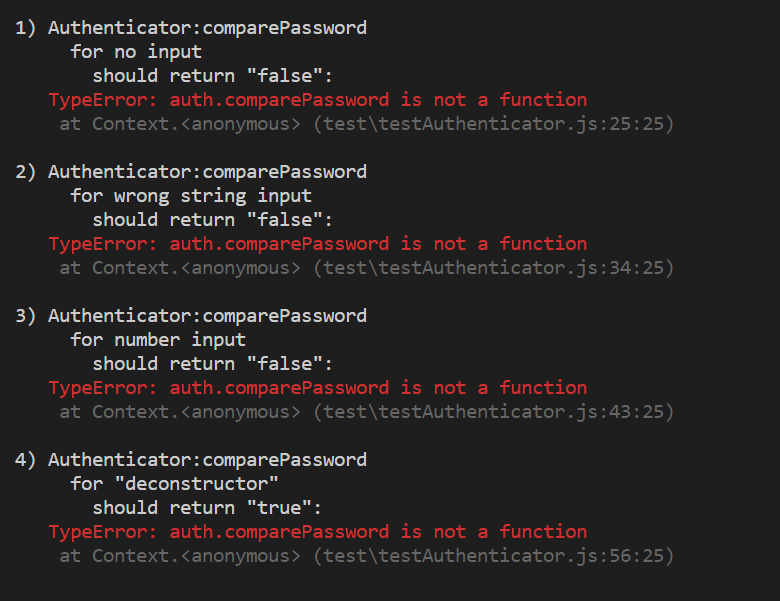
\includegraphics{authtest1.png}
	\caption{Test run for Authenticator before implementation}
\end{figure}
When the functionality had been implemented the test-run worked perfectly. See figure below.
\begin{figure}[H]\label{fig2}
	\centering
	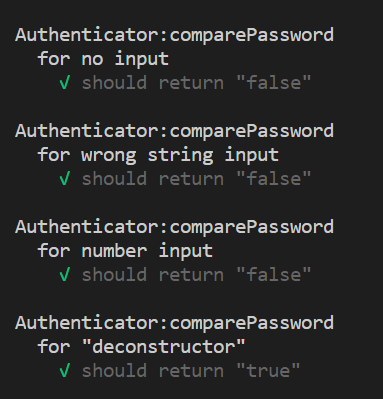
\includegraphics{authtest2.png}
	\caption{Test run for Authenticator after implementation}
\end{figure}

Next I needed to developed a method in the Word-class for generating a string showing the letters found and showing the position of the letters missing, e.g. if the word is "letter" and the letters not found are "e" and "t" the string should be shown in the following manner: "l \_ \_ \_ \_ r". Working with TDD I first created a test for the method to be developed. In the figure below the test has been run before implementation of the method.
\begin{figure}[H]\label{fig3}
	\centering
	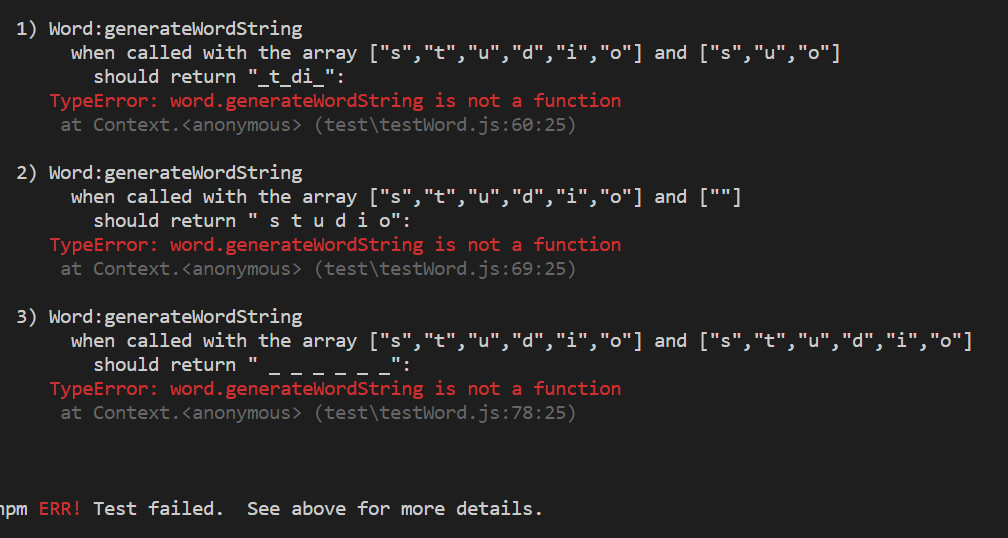
\includegraphics[scale=0.75]{wordtest1.png}
	\caption{Test run for "generateStringWord"-method before implementation}
\end{figure}
After having developed the function the test-run looks as follows. Thus, the method works as expected.
\begin{figure}[H]\label{fig4}
	\centering
	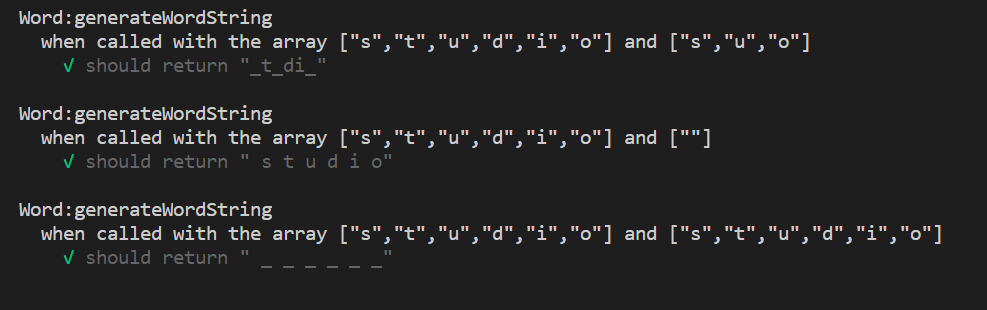
\includegraphics[scale=0.75]{wordtest2.png}
	\caption{Test run for "generateStringWord"-method after implementation}
\end{figure}
\subsubsection{Static and dynamic testing}
The code was tested statically using code review. The code was also tested dynamically by following the test-cases presented below (TC 3.1-3.3). These test-cases are also written in the document "test.pdf" for sake of completeness.
\subsubsection{TC 3.1 - Moving to managing words menu}
\begin{itemize}
	\item Name: Authenticating for managing words.
	\item Test case ref: TC 3.1
	\item Use case ref: UC 3
	\item Description: The test case tests how the system responds when the user tries to open the "manage words" menu.
\end{itemize}
\emph{Input}
\begin{enumerate}
	\item \underline{Precondition:} The user is located in the main menu.
	\item Select "Manage word." by using the cursor keys.
	\item Press enter.
\end{enumerate}
\emph{Expected}
\begin{itemize}
	\item The system prints "You need to be authenticated to manage words."
	\item The system prompts the user to "Input password:"
\end{itemize}
\emph{Comments}
No problems encountered.
\subsubsection{TC 3.2 - Inputting an incorrect password}
\begin{itemize}
	\item Name: Inputting an incorrect password.
	\item Test case ref: TC 3.2
	\item Use case ref: UC 3
	\item Description: The test case tests how the system responds when the user tries inputs an incorrect password when prompted for a password to move to the "manage words" menu.
\end{itemize}
\emph{Input}
\begin{enumerate}
	\item \underline{Precondition:} The user has selected "manage words" from the main menu and have been prompted by the system to input a password.
	\item Write "Frog"
	\item Press enter.
\end{enumerate}
\emph{Expected}
\begin{itemize}
	\item The system prints "Unfortunately the password was incorrect"
	\item The system displays the main menu.
\end{itemize}
\emph{Comments}
No problems encountered.
\subsubsection{TC 3.3 - Inputting a correct password}
\begin{itemize}
	\item Name: Inputting a correct password.
	\item Test case ref: TC 3.3
	\item Use case ref: UC 3
	\item Description: The test case tests how the system responds when the user tries inputs a correct password when prompted for a password to move to the "manage words" menu.
\end{itemize}
\emph{Input}
\begin{enumerate}
	\item \underline{Precondition:} The user has selected "manage words" from the main menu and have been prompted by the system to input a password.
	\item Write "deconstructor"
	\item Press enter.
\end{enumerate}
\emph{Expected}
\begin{itemize}
	\item The system displays the "Manage Words" menu.
\end{itemize}

\emph{Comments}
No problems encountered.
 
\subsection{Class diagram}
The class diagrams for the fully implemented game can be seen below. The class diagram can also be found in a separate file called "Class Diagram Final.pdf" in the folder "Use Cases".
\begin{figure}[H]\label{fig5}
	\centering
	\includegraphics[scale=0.5]{classdiagramfinal.png}
	\caption{Class diagram for the final implementation}
\end{figure}
\subsection{State machine}
I did a basic state machine for the authentication of the user trying to get access to the "manage words" menu. This state machine in shown below and can also be found in pdf-format in the folder "Use Cases" in the repository. The state machine is very simple since only two paths are available.
\begin{figure}[H]\label{fig6}
	\centering
	\includegraphics[scale=0.5]{statemachineauth.png}
	\caption{State Machine for the authentication step.}
\end{figure}
\subsection{Reflection}
This reflection regarding iteration 4 is also the final reflection of the document. For the final iteration I did not have much time. Therefore I choose to only implement a couple of features such that the game can be played and the words can be managed. I also had to do some bug because of problems with the implementation I found in iteration 3. I really liked the test-driven development methodology, so I tried to follow that method in this iteration. It is quite hard to first develop the tests, even for such simple functionality as I was developing here. But it is fun, and my (admittedly anecdotal and based on very limited data) opinion is that there is less bugs when working in this way. Most of the steps went faster in this iteration, which is understandable since I've already done them once. Even though I want to jump right into the coding I do feel that I now have more of a grasp of why this kind of deliberate development will be faster in the long run. One problem for me during the course was that even though we go through all the steps to develop the code in a deliberate manner I found that I wound up with a quite messy code. I think this is partly because I spent most focus on the actual documentation and the new concepts and I believe that in the long run this methodology will lead to better code and a more streamlined work process.

\section{Risk Analysis}
The overarching risks for this project is connected to the time available for performing the work. The possibility of a hardware failure is for example relatively low, especially considering the redundancy afforded by having two computers available. However, due to severe constraints regarding the time available all risks which reduces the available time are quite serious. Since all events will impact the time available they are all quite serious which make the most probable events most important (since both the impact and the probability are quite high). Thus, a lot of effort will have to be made to make sure that probable events are avoided or mitigated. The staff has children in pre-school which unfortunately equates to a lot of sickness. The probability that this event occurs is hard to reduce which is why the effect of such a event must be mitigated. In an effort to create somewhat of a buffer for these kind of events it is wise to try and keep ahead of schedule if possible.
\newline
\newline
Thus, the key risks have to do with estimations and people working within the project, both are risks in relation to the time available. There is no significant risk that changes to the software, as a response to management or costumer wishes, will need to be performed. The hardware risks are low as explained above. Since the application is a very basic application there are also no great risks in tools or technology changes impacting the development process. 
\subsection{List of risks}
Based on the above discussion a list of risks are presented below. Only risks which are deemed at all possible has been accounted for in the list. As can be seen, the risks are all related to the available time.
\begin{center}
	\begin{tabular}{|c|c|c|} 
		\hline
		Risk & Probability & Impact\\ [0.5ex] 
		\hline\hline
		Hardware failure & Low & Catastrophic \\ 
		\hline
		Illness & High & Serious \\
		\hline
		Underestimation of time requirements & Moderate & Serious \\ 
		\hline
		Too many features required in application & Moderate & Serious \\ 
		\hline
		
	\end{tabular}
\end{center}
\subsection{Strategies}
Since most of the risks are time-related the most prudent course of action is working ahead of schedule and use all time available. Thus, theory may e.g. be studied during transportation to and from events. Furthermore, in order to be use the available time efficiently it is important that the staff get good sleep and exercise regularly, which is why this is encouraged. This is a more general approach to utilization of the available time in an efficient manner. In the sections below each specific risk will be briefly addressed.
\subsubsection{Hardware failure}
Even though this risk is quite low it is still considered since such an event would be catastrophic. In order to reduce the likelihood of a hardware failure redundant systems are used (i.e. two computers). In the unlikely event of both systems failing a borrowed computer will have to do. This will of course be costly from a time-perspective but less so than having to buy a new computer.
\subsubsection{Illness}
This is a quite probable risk. Either that the developer himself falls ill or that his child do. The risk of the first scenario may be reduced by the measures described above as well as by eating healthy. To a certain point the same applies to the developers child. If the child would fall ill a fallback approach would be to enlist the help of other people to take care of the child and in that way increase the time for working on the project. Other remedies are of course medication in case of severe illness.
\subsubsection{Underestimation of time requirements}
This is a risk which is hard to reduce initially. However, as the project develops the time estimates may be adjusted based on experience. Thus, by minimizing the fault in the estimation the risk of the event happening will be lower. The risk may also be reduced by knowingly overestimating the time for each task by a certain factor, to create a buffer of sorts. If the time requirements have been greatly underestimated some requirements in the coming iterations may need to be scrapped in favor of essential requirements.
\subsubsection{Too many features required in application}
This risk is also quite probable and is mainly reduced by having a realistic approach in the planning stages. Prioritizing the requirements may be performed in order to let go of features which are not essential if it is determined that the time will not be enough for completing all the features. A core list of essential features must therefore be determined and prioritized during development. 
\subsection{Reflection}
I felt that performing the risk analysis was quite hard. For my specific situation, developing a quite basic application and having a very limited amount of time, it feels like the risk will always be related to time. If no direct costs are involved I guess the risk is almost always to complete the project in time (assuming that the project is possible to complete at all). This is very true here as well, especially considering the fact that the application is quite limited (in this sense it is not a risk that the application cannot be developed). I feel that risk analysis will be quite different in a large project, considering management, customers, budget etc. But this is still a healthy exercise I believe.

\end{document}          
